\documentclass[conference]{IEEEtran}

\usepackage{cite}
\usepackage{graphicx}
\usepackage{booktabs}
\usepackage{multirow}
\usepackage{amsmath}
\usepackage{siunitx}
\usepackage{hyperref}
\usepackage{xcolor}
\usepackage{algorithm}
\usepackage{algpseudocode}
\usepackage{tikz}
\usetikzlibrary{positioning,arrows.meta}

\title{Simulation-Driven Reinforcement Learning for Automated Penetration Testing:
Failure Diagnosis, Generalization, and Rapid Adaptation}

\author{\IEEEauthorblockN{Anonymous Authors}}

\begin{document}
\maketitle

\begin{abstract}
This paper presents a complete simulation-first study of reinforcement learning (RL) for automated penetration testing in a multi-subnet environment. We first identify and quantify a dead-loop pathology in off-policy value-based agents (DQN/DDQN), where scan idempotency induces repeated actions with no task progress. We then introduce an environment-level fix, recovering DQN/DDQN from 0\% success to 100\% in the fixed setting. Next, we evaluate out-of-distribution transfer on unseen network variants (X/Y/Z), where all original single-environment policies fail under zero-shot transfer. To improve transferability, we train generalized policies with randomized tasks and topology-aware observations, followed by few-shot adaptation. PPO and A2C reach 100\% success on all unseen variants under few-shot adaptation, while DQN remains structurally fragile on Y/Z. We additionally include DPPO-like and GAIL-like simulation extensions: DPPO-like reaches 100\% success with 3-step trajectories, while GAIL-like underperforms in this environment. Finally, we provide a reproducible real-experiment preparation pipeline (network specifications, runbooks, and execution logging templates) and explicitly separate simulation claims from live exploitation claims.
\end{abstract}

\begin{IEEEkeywords}
Reinforcement learning, automated penetration testing, simulation, generalization, few-shot adaptation, distributed PPO, imitation learning.
\end{IEEEkeywords}

\section{Introduction}
Automated penetration testing can be modeled as a sequential decision process where an agent must choose reconnaissance, exploitation, and lateral-movement actions to reach a crown-jewel host under constrained budgets. RL has been actively explored for this class of security automation tasks due to its ability to optimize long-horizon action sequences \cite{sutton2018,moerland2023}.

Despite this promise, two practical gaps remain. First, reward-design loopholes can induce pathological policies that maximize local reward while failing the mission objective. Second, policies trained on a single network often fail to generalize when topology or vulnerability mapping changes.

This work addresses both gaps with a complete experimental pipeline:
\begin{itemize}
    \item failure diagnosis and reward-structure fix,
    \item unseen-network transfer evaluation,
    \item generalized training and few-shot adaptation,
    \item extension to additional policy families (DPPO-like and GAIL-like),
    \item real-experiment preparation artifacts for future live execution.
\end{itemize}

\subsection{Contributions}
The main contributions are:
\begin{enumerate}
    \item \textbf{Dead-loop diagnosis and fix.} We identify repeated-scan dead loops in DQN/DDQN and show that scan-idempotency and re-exploit penalties recover learning behavior.
    \item \textbf{Transfer benchmark.} We construct unseen networks X/Y/Z and show complete zero-shot failure for original single-environment policies.
    \item \textbf{Adaptation pipeline.} We implement randomized task-family training with topology-aware observations and quantify few-shot adaptation gains.
    \item \textbf{Extended baselines.} We add DPPO-like and GAIL-like simulation agents and evaluate them in the same environment.
    \item \textbf{Reproducible preparation for live testing.} We release real-experiment network assets, execution configs, runbooks, and structured log templates.
\end{enumerate}

\section{Background}
RL foundations for sequential control are well established \cite{sutton2018}. In deep RL, value-based methods such as DQN \cite{mnih2015} and policy-gradient methods such as PPO \cite{schulman2017ppo} and A2C/A3C-style actor-critic variants \cite{mnih2016a3c} offer complementary trade-offs between sample efficiency and stability. Distributed PPO variants are commonly used in large-scale training systems.

Imitation learning and adversarial imitation (e.g., GAIL \cite{ho2016gail}) provide alternatives when expert trajectories are available. In security-oriented sequential domains, simulation is often necessary for safe and reproducible experimentation before live deployment. Our work focuses on this simulation-to-preparation stage, with explicit separation between simulation metrics and live exploitation claims.

\subsection{Representative Related Studies (10 Papers)}
We summarize ten representative studies that motivate our design choices and evaluation protocol.
\begin{enumerate}
    \item \textbf{Sutton and Barto (2018)}: formalized the MDP framework and core RL operators used by all methods in this paper \cite{sutton2018}.
    \item \textbf{Watkins and Dayan (1992)}: established Q-learning convergence in tabular settings, motivating our tabular baseline \cite{watkins1992}.
    \item \textbf{Mnih et al. (2015)}: introduced DQN with replay and target networks for high-dimensional value learning \cite{mnih2015}.
    \item \textbf{van Hasselt et al. (2016)}: proposed Double DQN to reduce overestimation bias in Q-value targets \cite{hasselt2016}.
    \item \textbf{Schulman et al. (2017)}: introduced PPO with clipped objectives for stable policy updates \cite{schulman2017ppo}.
    \item \textbf{Mnih et al. (2016)}: introduced A3C-style asynchronous actor-critic training for parallel experience collection \cite{mnih2016a3c}.
    \item \textbf{Lillicrap et al. (2016)}: proposed DDPG for continuous-control actor-critic learning with deterministic policies \cite{lillicrap2016}.
    \item \textbf{Ho and Ermon (2016)}: proposed GAIL, an adversarial framework for imitation from expert trajectories \cite{ho2016gail}.
    \item \textbf{Arulkumaran et al. (2017)}: synthesized deep RL design trade-offs and common instability modes \cite{arulkumaran2017}.
    \item \textbf{Moerland et al. (2023)}: surveyed RL for autonomous cyber defense and highlighted reproducibility and transfer gaps \cite{moerland2023}.
\end{enumerate}

\begin{table*}[t]
\centering
\caption{Comparison of ten representative related studies and their relevance to this paper.}
\label{tab:related-work-10}
\vspace{1mm}
\footnotesize{Rows are ordered by cyber-domain relevance first, followed by foundational RL works.}
\begin{tabular}{llllll}
\toprule
Reference & Primary Domain & Method Type & Main Contribution & Typical Limitation & Difference vs This Paper \\
\midrule
Moerland et al. (2023) \cite{moerland2023} & Cyber defense RL & Survey/benchmarking & Identified realism, transfer, and reproducibility gaps & Broad survey; limited controlled ablations & We provide controlled ablations, transfer tests, and reproducible artifacts in one pipeline. \\
Arulkumaran et al. (2017) \cite{arulkumaran2017} & Deep RL survey & Survey/analysis & Consolidated architectural and stability insights & Not focused on cyber-attack pipelines & We instantiate those insights in a cyber-attack simulation with measurable outcomes. \\
Sutton and Barto (2018) \cite{sutton2018} & General RL & Foundations & Unified RL formalism (MDP, TD, policy/value) & Not task-specific to cyber operations & We operationalize these principles for multi-subnet pentesting tasks. \\
Watkins and Dayan (1992) \cite{watkins1992} & General RL & Tabular value-based & Q-learning convergence analysis & Limited scalability in large state spaces & We retain tabular Q-learning only as a baseline against deep and actor-critic agents. \\
Mnih et al. (2015) \cite{mnih2015} & Deep RL control & Value-based (DQN) & Replay + target networks for deep Q-learning & Overestimation and reward-hacking sensitivity & We explicitly diagnose and fix reward-induced dead-loop behavior in this family. \\
van Hasselt et al. (2016) \cite{hasselt2016} & Deep RL control & Value-based (DDQN) & Reduced overestimation bias & Still sensitive to environment reward loopholes & We show that reducing overestimation alone is insufficient without environment-level reward safeguards. \\
Schulman et al. (2017) \cite{schulman2017ppo} & Deep RL control & Policy-gradient (PPO) & Stable clipped-policy optimization & On-policy sample cost can be high & We evaluate PPO under zero-shot transfer and few-shot adaptation on unseen networks. \\
Mnih et al. (2016) \cite{mnih2016a3c} & Deep RL control & Actor-critic (A3C) & Asynchronous parallel learning & Asynchrony can introduce optimization variance & We test an A3C-like baseline in the same benchmark for direct cross-family comparison. \\
Lillicrap et al. (2016) \cite{lillicrap2016} & Continuous control & Actor-critic (DDPG) & Deterministic policy gradients at scale & Brittle hyperparameter sensitivity & We include DDPG as a negative-result baseline under discrete pentesting dynamics. \\
Ho and Ermon (2016) \cite{ho2016gail} & Imitation learning & Adversarial imitation (GAIL) & Expert-distribution matching without explicit rewards & Requires high-quality demonstrations & We benchmark a GAIL-like variant and report its limits in this environment. \\
\bottomrule
\end{tabular}
\end{table*}

\subsection{Algorithm Primer}
For readability, we summarize the role of each algorithm family used in this study.
\begin{itemize}
    \item \textbf{Q-Learning}: tabular value iteration over state-action pairs; useful as a low-dimensional baseline for convergence behavior and reward-shaping sensitivity \cite{sutton2018}.
    \item \textbf{DQN/DDQN}: neural value approximation for larger state spaces; DDQN reduces overestimation bias by decoupling action selection and target evaluation \cite{mnih2015}. In our task, these methods are especially sensitive to reward loopholes.
    \item \textbf{PPO}: clipped policy-gradient optimization that stabilizes actor updates while preserving sample efficiency; widely used as a robust default for continuous and discrete control \cite{schulman2017ppo}.
    \item \textbf{A2C/A3C-like}: advantage actor-critic methods that jointly learn policy and value, with asynchronous or parallelized rollout collection for improved training throughput \cite{mnih2016a3c}.
    \item \textbf{DPPO-like}: distributed PPO surrogate used here to scale on-policy data collection in vectorized environments; conceptually aligned with PPO but focused on parallel rollout efficiency.
    \item \textbf{GAIL-like}: adversarial imitation that trains a policy to match expert trajectory distributions via discriminator feedback; effective when expert demonstrations are informative and diverse \cite{ho2016gail}.
\end{itemize}

\subsection{Reference Sources}
All cited background papers are linked in the bibliography with source URLs or DOI landing pages (see \texttt{references.bib}) to make paper lookup and verification straightforward.

\subsection{Environment and Experimental Setup}
\subsection{Complex Simulation Environment}
We use a 6-host, 3-subnet environment (DMZ, Internal, Core) with 30 discrete actions:
\begin{equation}
|\mathcal{A}| = N_{hosts} \times (1 + N_{exploit\_families}) = 6 \times 5 = 30.
\end{equation}

Each host state contains discovery, exploitation, and vulnerability-indicator bits. The mission objective is to compromise the crown-jewel host within a fixed horizon.

\begin{figure}[t]
    \centering
    \begin{tikzpicture}[
        node distance=0.6cm and 0.75cm,
        box/.style={draw, rounded corners, minimum width=1.35cm, minimum height=0.55cm, align=center, font=\scriptsize},
        zone/.style={draw, dashed, rounded corners, inner sep=5pt}
    ]
        \node[box] (atk) {Attacker};

        \node[box, right=1.5cm of atk] (dmz1) {DMZ-H1};
        \node[box, below=0.35cm of dmz1] (dmz2) {DMZ-H2};

        \node[box, right=1.9cm of dmz1] (int1) {INT-H3};
        \node[box, below=0.35cm of int1] (int2) {INT-H4};

        \node[box, right=1.9cm of int1] (core1) {CORE-H5};
        \node[box, below=0.35cm of core1] (core2) {CORE-H6\\(Goal)};

        \draw[-{Stealth[length=2mm]}] (atk) -- (dmz1);
        \draw[-{Stealth[length=2mm]}] (atk) -- (dmz2);
        \draw[-{Stealth[length=2mm]}] (dmz1) -- (int1);
        \draw[-{Stealth[length=2mm]}] (dmz2) -- (int2);
        \draw[-{Stealth[length=2mm]}] (int1) -- (core1);
        \draw[-{Stealth[length=2mm]}] (int2) -- (core2);

        \node[zone, fit=(dmz1)(dmz2), label=above:{\scriptsize DMZ}] {};
        \node[zone, fit=(int1)(int2), label=above:{\scriptsize Internal}] {};
        \node[zone, fit=(core1)(core2), label=above:{\scriptsize Core}] {};
    \end{tikzpicture}
    \caption{Representative multi-subnet topology used in simulation: attacker entry through DMZ, pivot through Internal, and objective in Core.}
    \label{fig:topology-overview}
\end{figure}

\subsection{Reward Structure}
The reward includes per-step cost, scan reward, pivot reward, terminal success reward, and penalties for blocked or incorrect actions. We tested:
\begin{itemize}
    \item \textbf{Original environment}: scan action remained positively rewarding under repetition.
    \item \textbf{Fixed environment}: redundant scans and re-exploits are penalized.
\end{itemize}

\subsection{Agents and Training}
Primary agents: Random, Deterministic HARMer, Q-Learning, PPO, DQN, DDQN, A2C, DDPG, and A3C-like.

Extensions:
\begin{itemize}
    \item \textbf{DPPO-like}: vectorized PPO surrogate for distributed rollouts.
    \item \textbf{GAIL-like}: adversarial imitation from oracle demonstrations in simulation.
\end{itemize}

All reported comparison metrics are from 30 evaluation episodes per agent unless stated otherwise.

\section{Proposed Work}
\subsection{Dead-Loop Suppression}
We observed that DQN/DDQN policies learned to repeatedly scan already-scanned nodes, producing high local reward with no objective progress. We introduced two penalties:
\begin{itemize}
    \item scan idempotency penalty,
    \item stronger re-exploit penalty.
\end{itemize}

This environment-level regularization altered trajectory incentives and removed the dominant degenerate loop.

\subsection{Generalization and Adaptation Protocol}
We define three unseen networks (X/Y/Z) that perturb vulnerability assignment and/or pivot constraints. Evaluation proceeds in two phases:
\begin{enumerate}
    \item zero-shot transfer from source-trained policies,
    \item few-shot adaptation with limited additional updates on target networks.
\end{enumerate}

\subsection{Simulation-Only DPPO/GAIL Integration}
DPPO-like was implemented via vectorized PPO training. GAIL-like used oracle-generated demonstrations and adversarial discriminator-guided policy optimization. Both are used as simulation baselines and not as live exploit controllers.

\subsection{Simplified Pseudocode}
Algorithm~\ref{alg:train} summarizes the training loop shared by our RL baselines. Algorithm~\ref{alg:transfer} summarizes the transfer and few-shot adaptation protocol used for X/Y/Z.

\begin{algorithm}[t]
\caption{Simulation RL Training (Simplified)}
\label{alg:train}
\begin{algorithmic}[1]
\State Initialize policy/value parameters $\theta$
\For{each training episode}
    \State Reset environment and obtain initial state $s_0$
    \For{$t = 0$ to horizon $T$}
        \State Select action $a_t$ from policy (or $\epsilon$-greedy for value methods)
        \State Execute $a_t$, observe reward $r_t$ and next state $s_{t+1}$
        \State Store transition and update parameters $\theta$
        \If{goal host is compromised}
            \State \textbf{break}
        \EndIf
    \EndFor
\EndFor
\State Return trained policy
\end{algorithmic}
\end{algorithm}

\begin{algorithm}[t]
\caption{Transfer + Few-Shot Adaptation (Simplified)}
\label{alg:transfer}
\begin{algorithmic}[1]
\State Train base policy on source task family
\For{each unseen target network $n \in \{X,Y,Z\}$}
    \State Evaluate zero-shot success of base policy on $n$
    \State Run limited adaptation updates on $n$
    \State Re-evaluate adapted policy on $n$
    \State Log success rate, reward, and average steps
\EndFor
\State Compare zero-shot vs few-shot performance
\end{algorithmic}
\end{algorithm}

\section{Evaluation}
\subsection{Main Simulation Results}
The evaluation follows the topology in Fig.~\ref{fig:topology-overview} and the procedures in Algorithm~\ref{alg:train} and Algorithm~\ref{alg:transfer}, enabling direct mapping from environment assumptions to reported metrics.

Table~\ref{tab:main-sim} and Fig.~\ref{fig:sim-main} report final simulation performance including DPPO-like and GAIL-like.

\begin{table}[t]
\centering
\caption{Main simulation results on the complex environment (30 episodes).}
\label{tab:main-sim}
\begin{tabular}{lccc}
\toprule
Agent & Success (\%) & Mean Reward & Avg Steps \\
\midrule
Random & 63.3 & 15.32 & 38.2 \\
Deterministic HARMer & 100.0 & 201.00 & 22.0 \\
Q-Learning & 100.0 & 247.00 & 6.0 \\
PPO & 100.0 & 247.00 & 6.0 \\
DQN & 0.0 & 114.00 & N/A \\
DDQN & 0.0 & 98.00 & N/A \\
A2C & 100.0 & 247.00 & 6.0 \\
DDPG & 0.0 & -62.00 & N/A \\
A3C-like & 100.0 & 218.50 & 3.0 \\
DPPO-like & 100.0 & 218.50 & 3.0 \\
GAIL-like & 0.0 & -79.00 & N/A \\
\bottomrule
\end{tabular}
\end{table}

\begin{figure}[t]
    \centering
    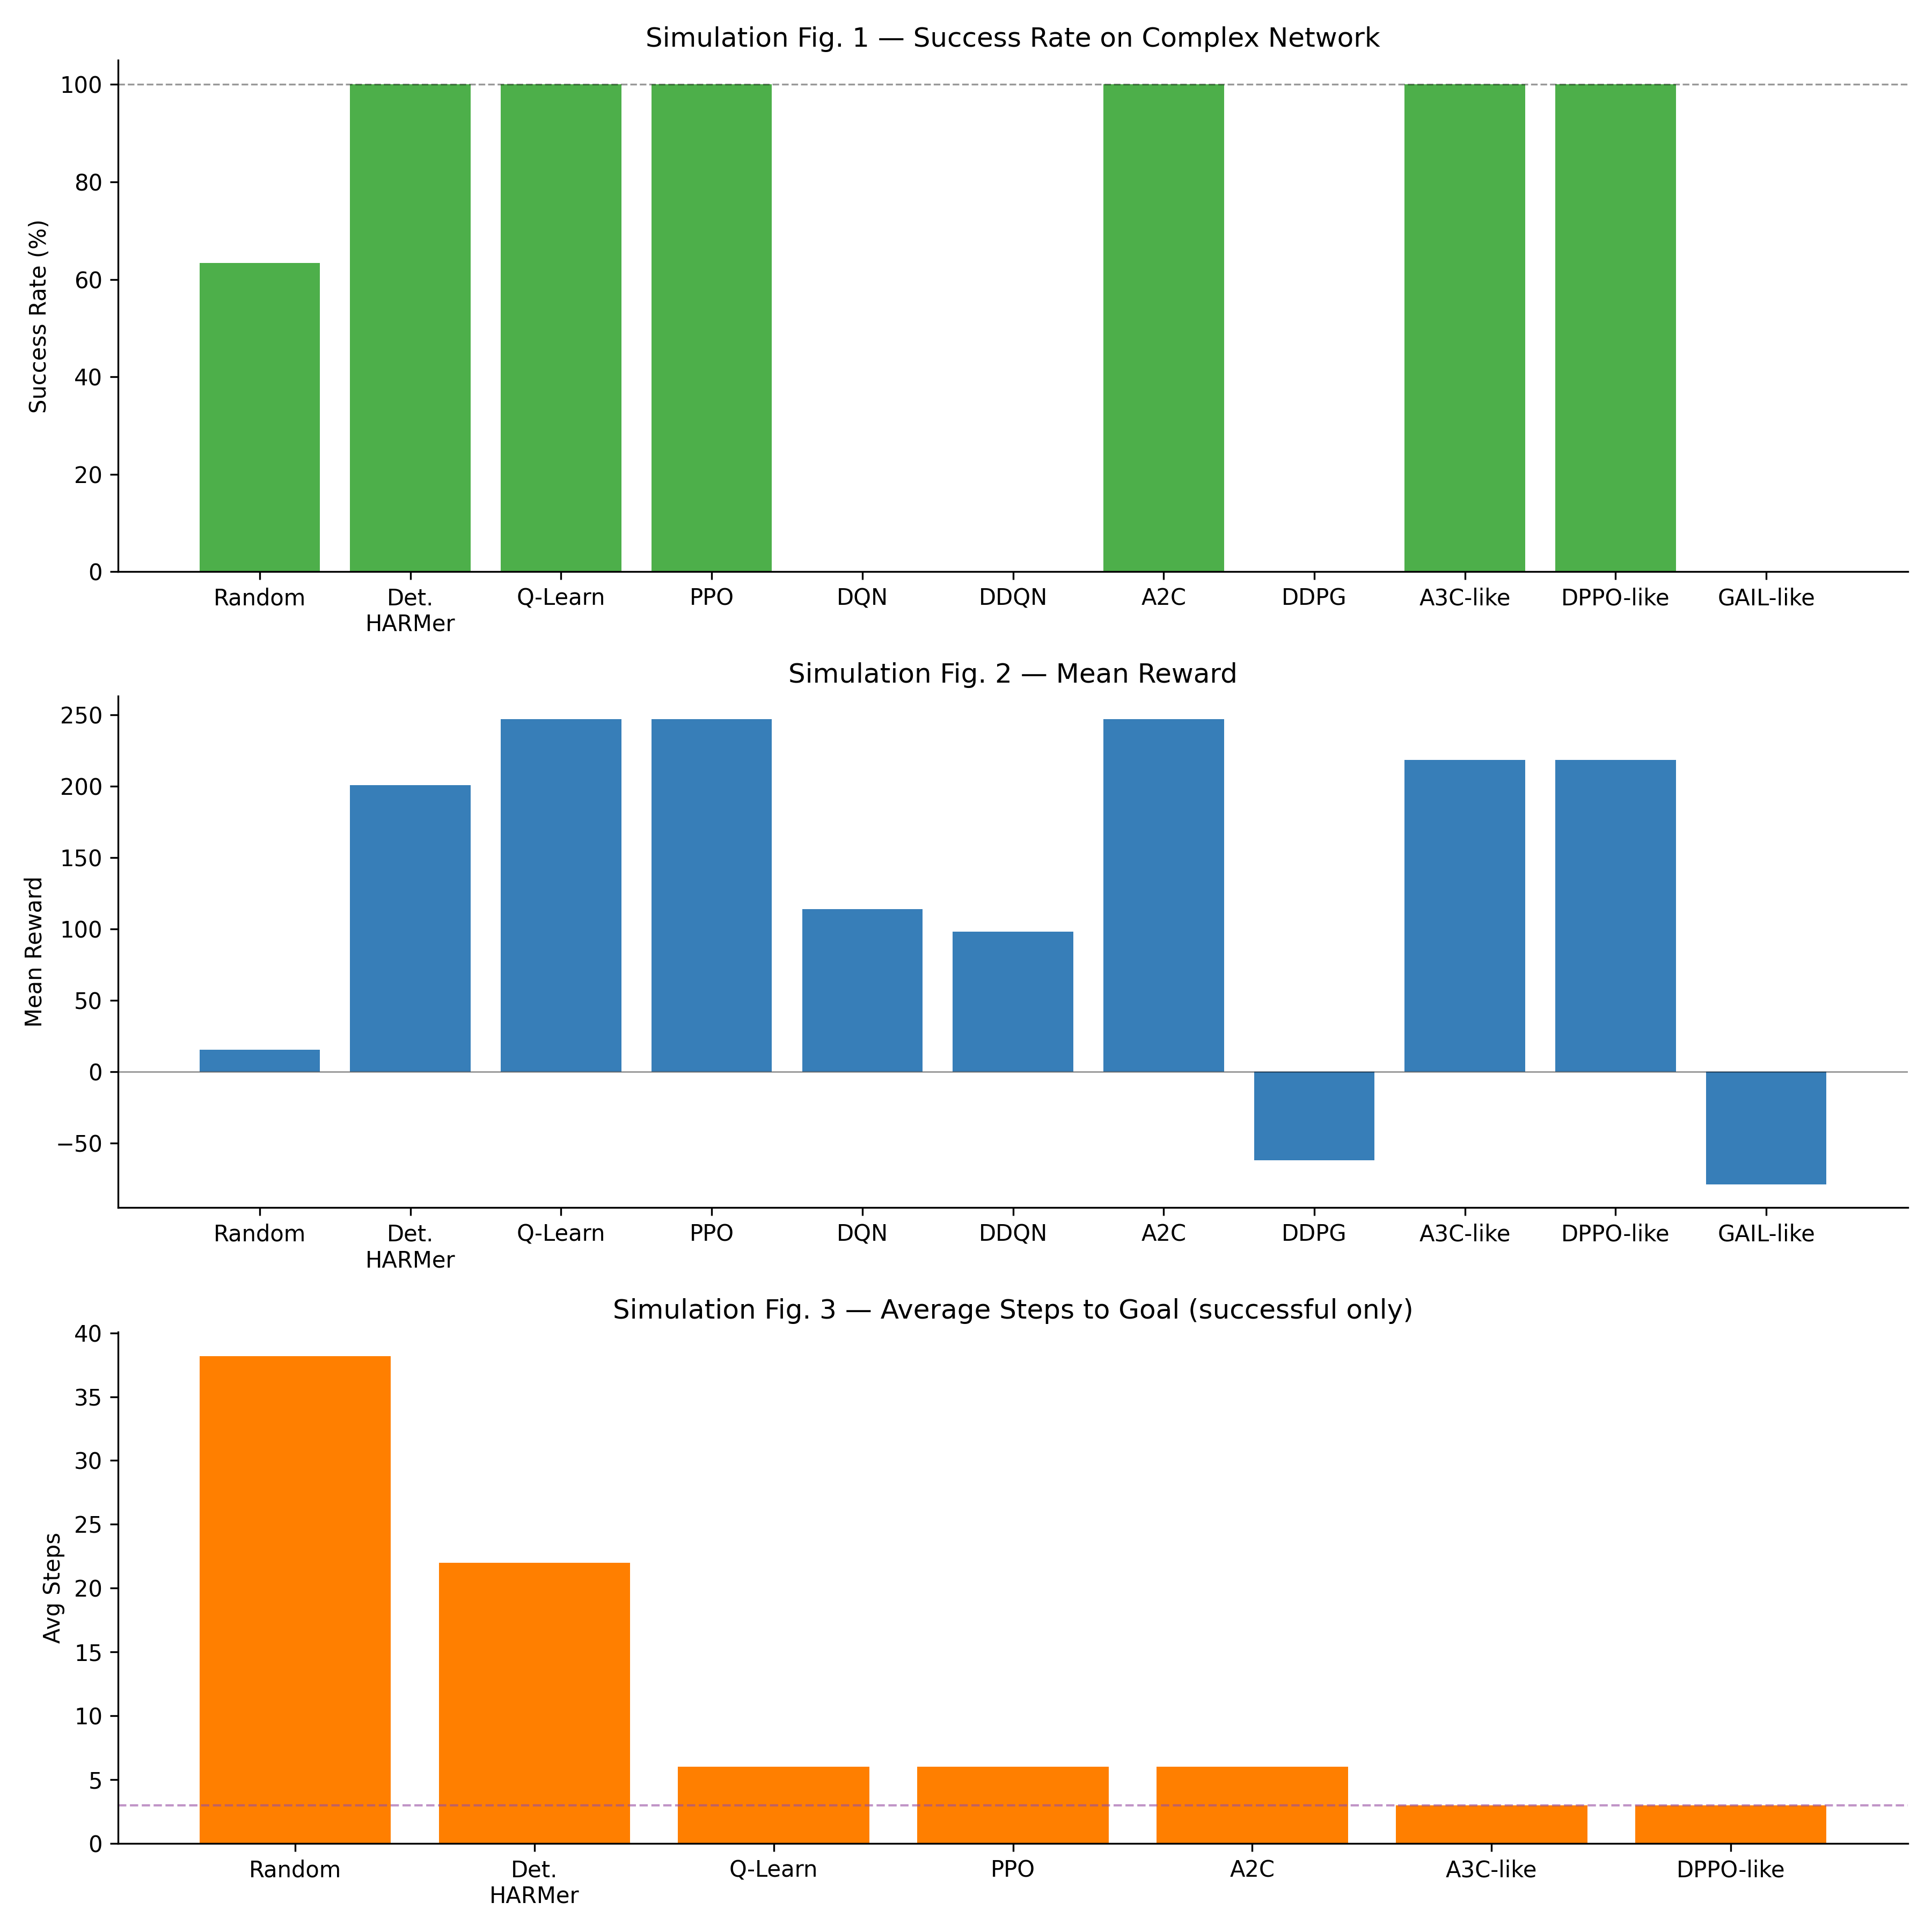
\includegraphics[width=0.98\linewidth]{figures/simulation_fig_main.png}
    \caption{Simulation summary over all evaluated agents: success, reward, and efficiency.}
    \label{fig:sim-main}
\end{figure}

\subsection{Effect of Environment Fix}
In the original environment, DQN/DDQN both reached 0\% success despite nontrivial rewards, consistent with scan-loop exploitation. Under fixed rewards, both methods recovered to 100\% success in prior fixed-environment experiments, confirming that the dominant failure mode was reward-structure-induced.

\subsection{Transfer and Few-Shot Adaptation}
Table~\ref{tab:adapt} and Fig.~\ref{fig:transfer-adapt} summarize unseen-network behavior. Original zero-shot transfer failed across X/Y/Z. With generalized training and few-shot adaptation, PPO/A2C achieved robust success; DQN remained brittle on Y and Z.

\begin{table}[t]
\centering
\caption{Generalization and few-shot adaptation on unseen networks.}
\label{tab:adapt}
\begin{tabular}{lcccc}
\toprule
Network & Agent & Zero-shot SR (\%) & Few-shot SR (\%) & Few-shot Steps \\
\midrule
X & PPO & 0 & 100 & 3.0 \\
X & A2C & 0 & 100 & 3.0 \\
X & DQN & 0 & 100 & 3.0 \\
Y & PPO & 0 & 100 & 3.0 \\
Y & A2C & 0 & 100 & 3.0 \\
Y & DQN & 0 & 0 & N/A \\
Z & PPO & 0 & 100 & 4.0 \\
Z & A2C & 0 & 100 & 4.0 \\
Z & DQN & 0 & 0 & N/A \\
\bottomrule
\end{tabular}
\end{table}

\begin{figure}[t]
    \centering
    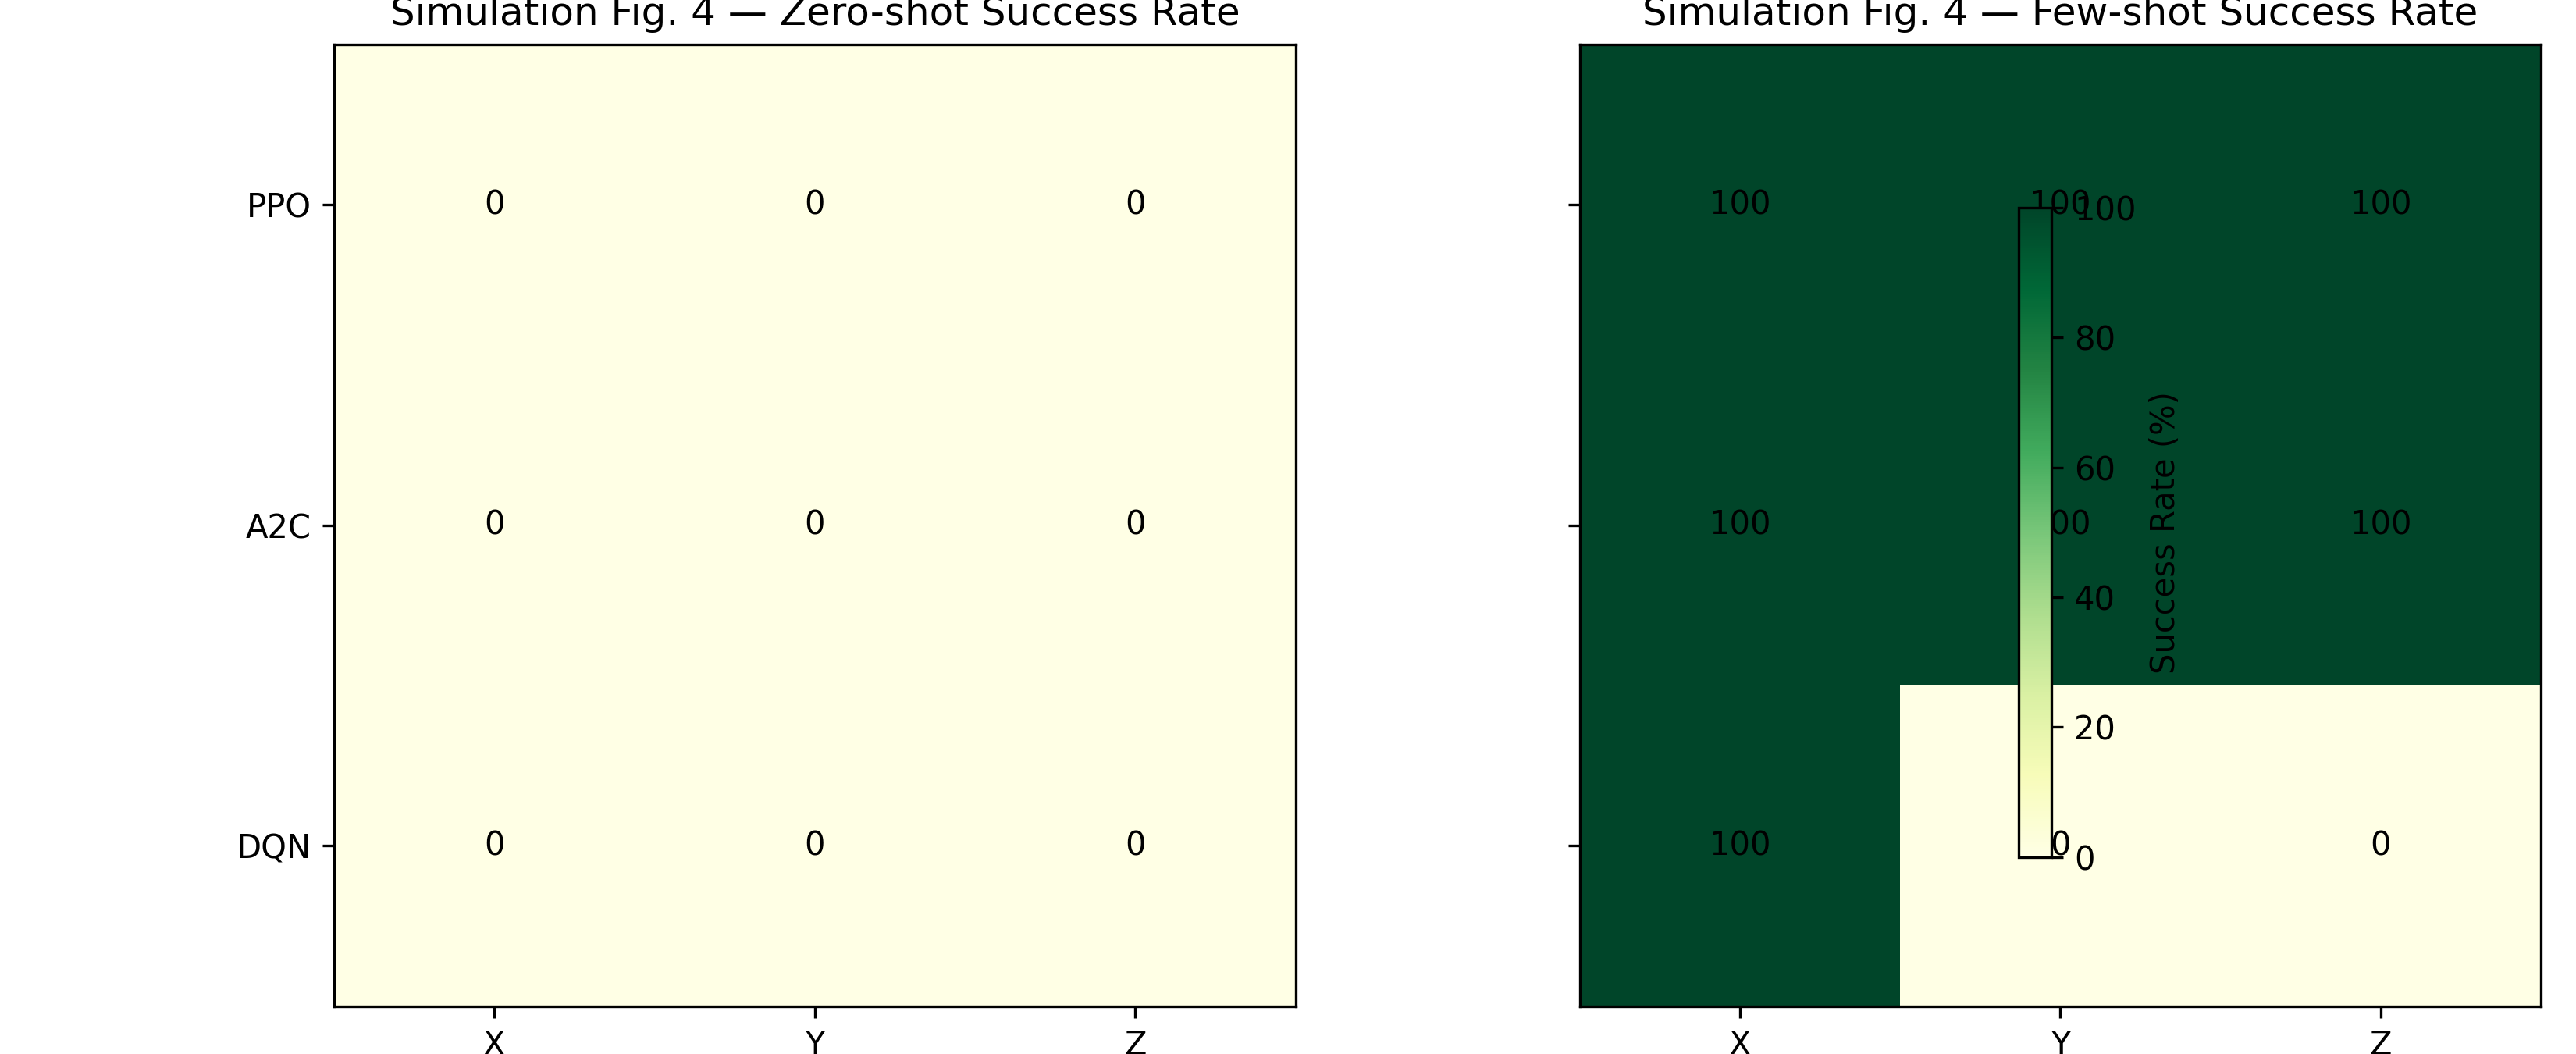
\includegraphics[width=0.95\linewidth]{figures/simulation_fig_transfer_adaptation.png}
    \caption{Success-rate heatmaps for zero-shot and few-shot adaptation on X/Y/Z.}
    \label{fig:transfer-adapt}
\end{figure}

\subsection{Real-Experiment Preparation and Dry-Run Validation}
We prepared four real-experiment network assets (alpha, beta, gamma, delta) and executed a structured dry-run over all four. Each dry-run validates configuration and runbook paths without performing any live network operation. Exploitation stages are explicitly logged as \texttt{skipped}.

Each network asset includes:
\begin{itemize}
    \item network JSON specification (subnet topology, host IPs, vulnerability hints),
    \item execution config (target host, attacker entry subnet, objective),
    \item runbook (ordered attack-path steps),
    \item structured CSV/JSON execution log (per-stage status, timestamp, session flag).
\end{itemize}

Table~\ref{tab:real-prep} summarizes the network complexity and Table~\ref{tab:real-dryrun} reports the dry-run stage outcomes for all four networks.
Fig.~\ref{fig:real-prep} visualizes the network characteristics.

\begin{table}[t]
\centering
\caption{Real-experiment network specifications.}
\label{tab:real-prep}
\begin{tabular}{lcccc}
\toprule
Network & Subnets & Hosts & Reachability Rules & Decoy \\
\midrule
alpha & 3 & 6 & 2 & no \\
beta  & 3 & 6 & 2 & no \\
gamma & 3 & 6 & 2 & no \\
delta & 4 & 6 & 4 & yes \\
\bottomrule
\end{tabular}
\end{table}

\begin{table}[t]
\centering
\caption{Dry-run execution stage outcomes across all four networks (total 39 log rows).}
\label{tab:real-dryrun}
\begin{tabular}{lcccc}
\toprule
Network & Preflight & Docker & MSF RPC & Exploit / Lateral \\
\midrule
alpha & \textbf{ok} & skipped & skipped & skipped \\
beta  & \textbf{ok} & skipped & skipped & skipped \\
gamma & \textbf{ok} & skipped & skipped & skipped \\
delta & \textbf{ok} & skipped & skipped & skipped \\
\bottomrule
\multicolumn{5}{l}{\footnotesize Skipped = not executed (dry-run); no live exploitation performed.}
\end{tabular}
\end{table}

\begin{figure}[t]
    \centering
    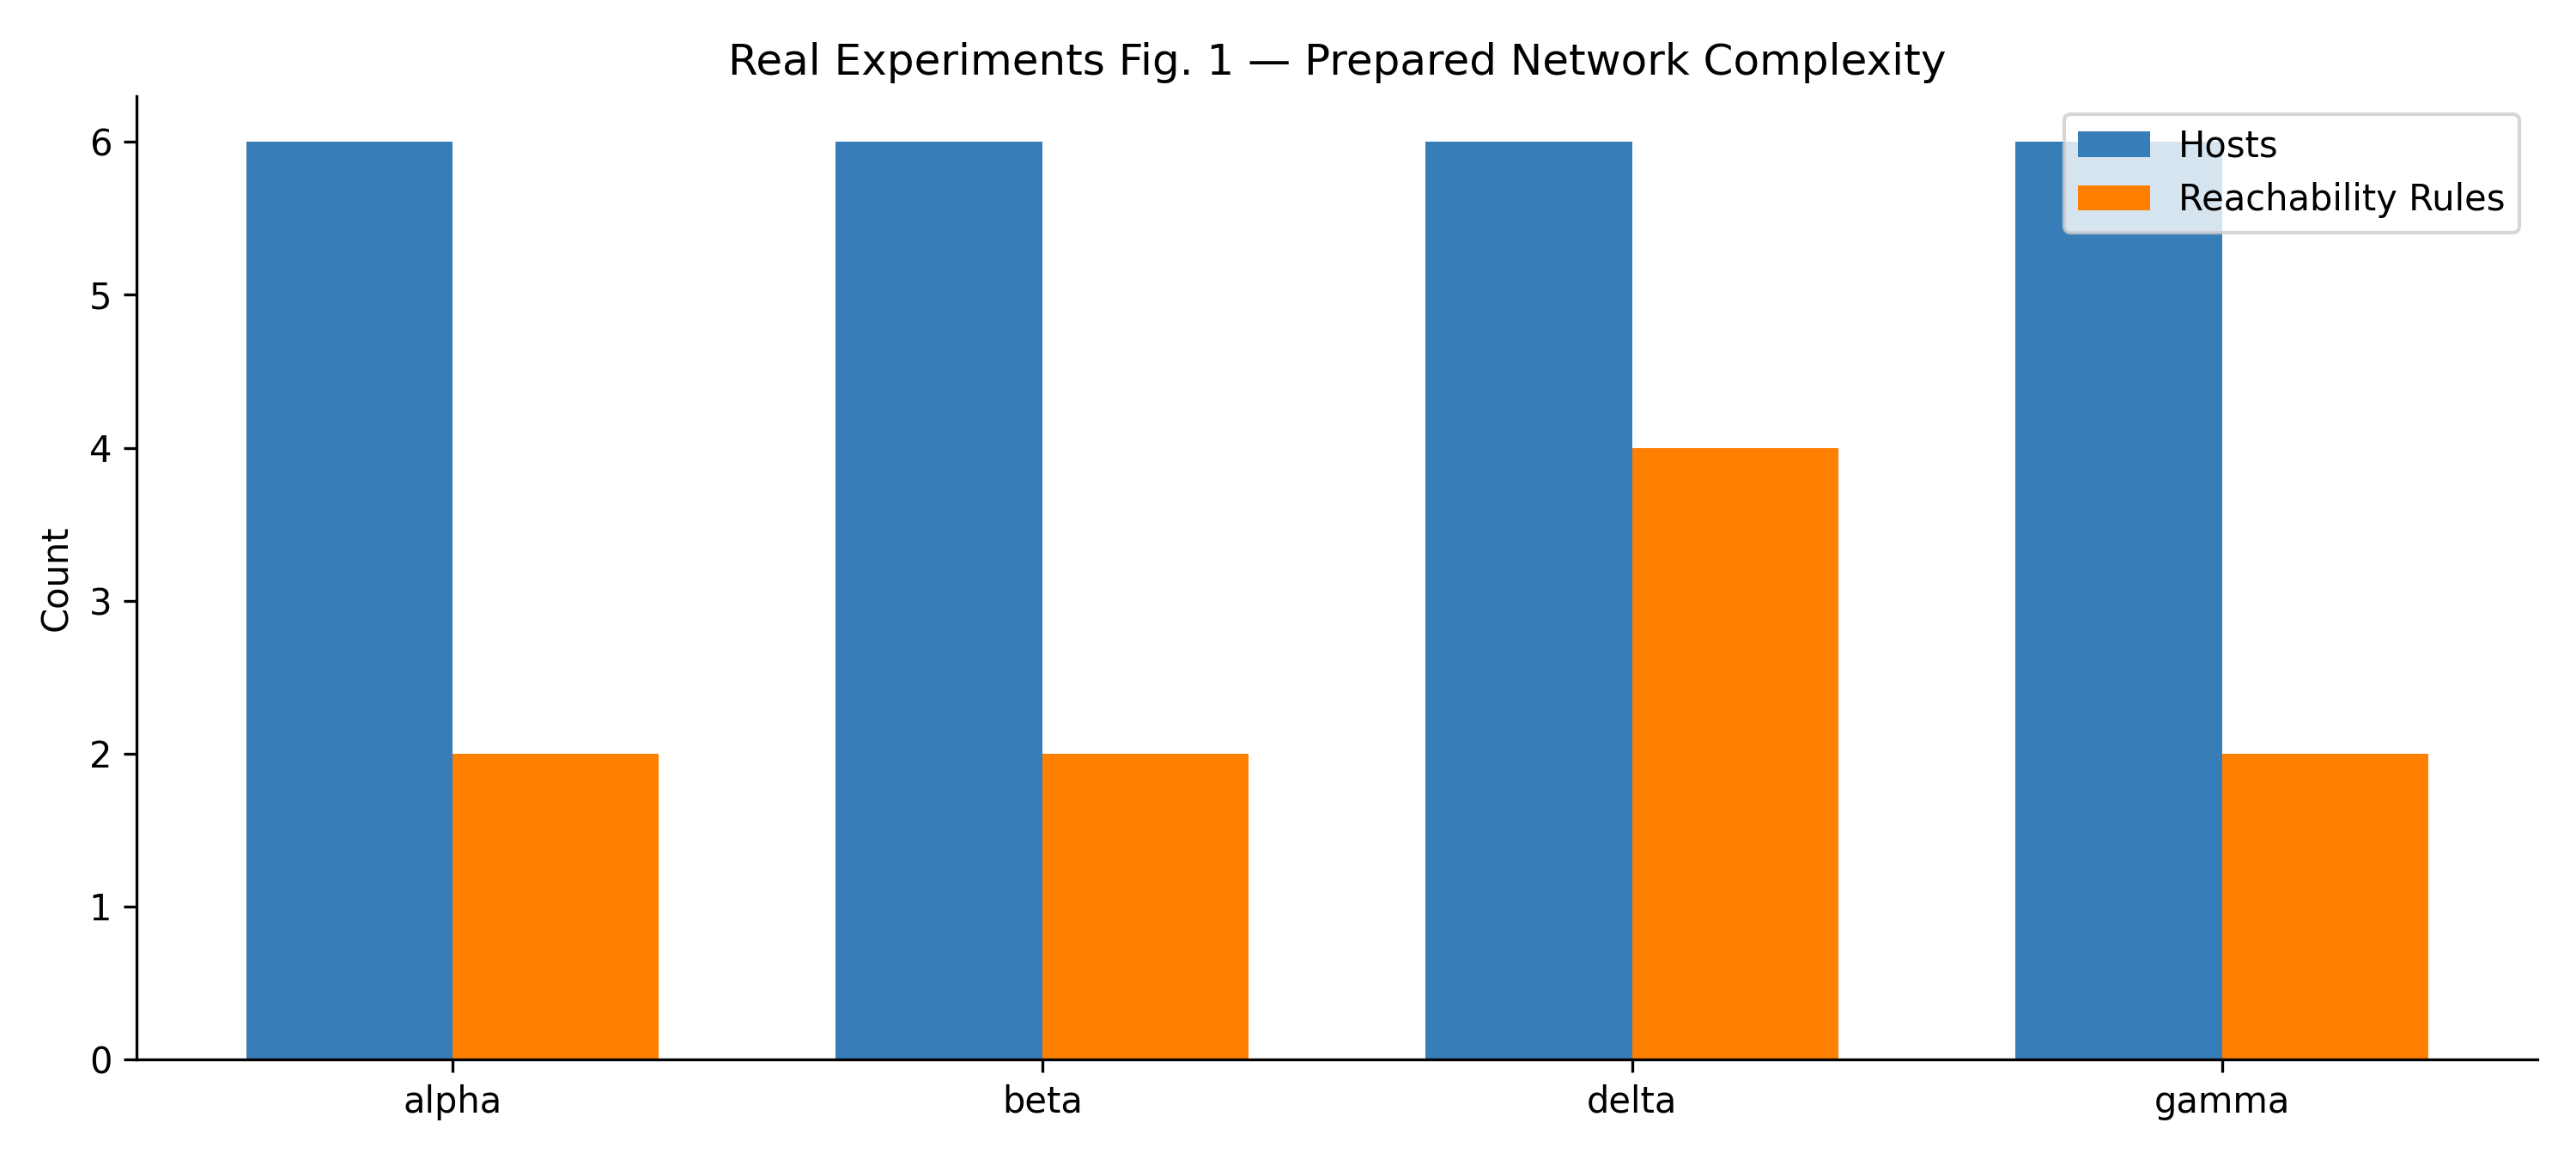
\includegraphics[width=0.90\linewidth]{figures/real_experiments_preparation_summary.png}
    \caption{Prepared network complexity: subnet count, reachability rules, and decoy presence.}
    \label{fig:real-prep}
\end{figure}

\section{Discussion}
We highlight four key findings.

\textbf{F1: Reward loopholes can dominate policy learning.}
Off-policy value methods are sensitive to idempotent local rewards; environment design must prevent profitable no-progress loops.

\textbf{F2: Single-environment training does not imply transfer.}
Zero-shot failure across X/Y/Z confirms strong overfitting to source-network semantics.

\textbf{F3: Few-shot adaptation is practically effective.}
Generalized pretraining plus few-shot adaptation recovers strong performance for PPO/A2C.

\textbf{F4: DPPO-like is strong in this environment; GAIL-like is not yet robust.}
In our setup, distributed PPO surrogate reaches optimal short trajectories, while adversarial imitation requires further trajectory coverage and regularization improvements.

\subsection{Threats to Validity}
\subsection{Internal Validity}
Simulation dynamics are deterministic and stylized; some effects may be amplified relative to live networks.

\subsection{External Validity}
Although we introduced unseen variants and randomized training, scale remains modest (6 hosts per core benchmark). Transfer conclusions should be interpreted within this controlled scope.

\subsection{Construct Validity}
``Success'' is defined as reaching the simulated crown-jewel state. This proxy does not yet include operational constraints such as stealth or detection evasion.

\subsection{Ethical Scope and Safety Statement}
This manuscript reports simulation results and preparation artifacts. It does not claim live compromise.

For the reported metrics, the following actions were \textbf{not performed}:
\begin{itemize}
    \item Docker container access,
    \item Metasploit RPC invocation,
    \item exploit module execution,
    \item payload delivery,
    \item shell/session acquisition,
    \item real service fingerprinting,
    \item real lateral movement.
\end{itemize}

Live testing, if conducted later, should be restricted to explicitly authorized lab environments.

\section{Conclusion}
We provided a complete simulation pipeline from diagnosis to adaptation and extended baselines. The results support two practical recommendations: (i) incorporate reward-level safeguards against no-progress loops, and (ii) evaluate robustness via transfer and few-shot adaptation rather than source-environment performance only.

Future work includes graph-native policy architectures, richer adversarial imitation setups, and controlled transition from prepared real-experiment assets to live validation.

\subsection*{Artifact and Reproducibility Notes}
The draft uses repository-generated files:
\begin{itemize}
    \item \texttt{results\_compare\_complex\_simulation.csv}
    \item \texttt{results\_transfer\_xyz.csv}
    \item \texttt{results\_generalization\_adaptation.csv}
    \item \texttt{real\_experiments/results/real\_experiments\_preparation\_summary.csv}
\end{itemize}

\bibliographystyle{IEEEtran}
\bibliography{references}

\end{document}
